\chapter{Generalized frequency division multiplexing single input single output}\label{sec:GFDMSISO}
\section{System model}\label{part:SMSISO}
In this subsection will be explained the system model for the GFDM . We consider the system where transmitted signal is sent through the channel. The channel in physical meaning is the number of multipath propagation components from transmitter to the receiver or the convolution of the transmitted signal with some channel profile.  We  explain the received signal as matrix product between convolution matrix and the transmitted data array \eqref{siso_1}, where $\mathbf{y}$ is received array, $\mathbf{x}$ is transmitted array and $\mathbf{H}$ is channel convolution matrix. The  different channel models are considered in the thesis\eqref{siso_2}\eqref{siso_3}\cite{Book21}.
\begin{align}
\mathbf{y}=\mathbf{Hx}
\label{siso_1}
\end{align}
\begin{align*}
\mathbf{y,x}\in\compl^{T\times 1}
\mathbf{H}\in\compl^{T\times T}
\end{align*}
\begin{align}
\mathbf{x}=\mathcal{X}_{[3]}=vec(\mathcal{X})=\mathbf{\Omega}_1 vec(\mathbf{S})
\label{siso_2}
\end{align}
\begin{align*}
\mathbf{\Omega}_1 \in \compl^{T\times T_s \cdot F}
\end{align*}
\begin{align}
\mathbf{\Omega}_1=(\mathbf{C}^{[b]T}\diamond \mathbf{C}^{[a]T})^T \diamond (\mathbf{b^T \otimes a}) \
\end{align}
\begin{align}
\mathcal{X}_{:,:,i}=\mathbf{a}\cdot diag(\mathbf{C}^{[a]}_{:,i})\cdot \mathbf{S} \cdot diag(\mathbf{C}^{[b]}_{:,i}) \cdot \mathbf{b} \label{siso_3}
\end{align}
The transmitted data is the third order PARATUCK2 tensor in the vectorized or unfolding form. The symbol matrix $\mathbf{S}$ introduced as the core matrix in the PARATUCK2 model\cite{Book6}. The symbols are written in the core matrix without any correction.
 Each column in the $\mathbf{C^{[a]}}$ matrix corresponds to the certain sub-carrier frequency for the stream modulation\eqref{siso_4}\eqref{siso_5}.The $\mathbf{C^{[a]}}$ matrix is constructed as the sub-carrier frequency  time samples in the each column, where column $i$ will correspond to the $i$ sub-carrier in the GFDM system. The overall equation to the $\mathbf{C^{[a]}}$ construction is explained in the \eqref{siso_1}. 
 \begin{align}
 c^{[a]}_{t,f}=e^{-j2\pi\cdot(t\cdot f)/T_s} \label{siso_4}
 \end{align}
\begin{align}
\mathbf{C}^{[a]}=\begin{bmatrix}
e^{-j2\pi\cdot 0}& e^{-j2\pi\cdot 0}& \cdots & e^{-j2\pi\cdot 0} \\
e^{-j2\pi\cdot 0}& e^{-j2\pi\cdot 1/T_s}& \cdots &e^{-j2\pi\cdot F/T_s} \\
e^{-j2\pi\cdot 0}& e^{-j2\pi\cdot 2/T_s}& \cdots &e^{-j2\pi\cdot 2F/T_s} \\
&&\vdots \\
e^{-j2\pi\cdot 0}& e^{-j2\pi\cdot T/T_s}& \cdots & e^{-j2\pi\cdot T\cdot F /T_s} \\
\end{bmatrix} \label{siso_5}
\end{align}
 Each column in the $\mathbf{C^{[b]}}$ define spread of the certain symbol over the all transmission block \eqref{siso_6}\cite{Book12}.  Elements in the columns are the time filter functions for the symbols. Each column is the shifted version of the other. The shift between near columns is equal to the $ T/T_s$ \eqref{siso_7}. The time filters functions are the root-raised cosine filter with adjustable $\alpha$ coefficient.
\begin{align}
\begin{matrix}
u(t) &=& \left\{ \begin{matrix} 
\frac{1-\alpha +4\alpha/\pi}{\sqrt{T}}& if& t=0\\
\frac{\alpha}{\sqrt{2T}}[(1+\frac{2}{\pi})sin(\frac{\pi}{4\alpha})+(1-\frac{2}{\pi})cos(\frac{\pi}{4\alpha})] & if &t= \pm T/4\alpha\\
\frac{1}{\frac{t\pi}{\sqrt{T}}(1-\frac{4*\alpha t}{T})^2}(sin(\frac{\pi t (1-\alpha)}{T})+\frac{4\alpha t}{T} cos(\frac{\pi t (1+ \alpha)}{T}) ) &otherwise \\
\end{matrix} \right.
\end{matrix}\label{siso_6}
\end{align}
\begin{align}
\mathbf{C}^{[b]}=\begin{bmatrix}
\mathbf{u}_{0}& \mathbf{u}_{1}& \cdots &\mathbf{u}_{T_s}\\
\end{bmatrix} \label{siso_7}
\end{align}
 The  $\mathbf{B}$ matrix become $\mathbf{b}$ array
and in the physical meaning corresponds to the time variation inside the one transmission block for different symbols or as selection coefficients for the different time slots\cite{Book34}.  We assume that system is linear time invariant and therefore $\mathbf{b}$ become array with all-ones structure \eqref{siso_8}.
\begin{align}
\mathbf{b}=\mathbf{1}_{T_s\times 1} \label{siso_8}
\end{align}
\begin{align}
\mathbf{b}\in \real^{T_s\times 1} \label{siso_9}
\end{align}
The  $\mathbf{A}$ matrix become $\mathbf{a}$ array and in the physical meaning corresponds to the transmission coefficient for each sub-carrier frequency stream or  selection array for sub-carriers inside of the one transmission block \eqref{siso_10}. We will consider the system where the $\mathbf{a}$ will have two typical structures. First is the array with all-ones in case if there is no overlapping in the frequency domain systems and known to the receiver. In the second case the values in the $\mathbf{a}$ is unknown for the receiver and have random variables from the range $[0,1]$
\begin{align}
\mathbf{a}=\mathbf{1}_{1\times F} \label{siso_10}
\end{align}
\begin{align}
\mathbf{a}\in \compl^{1\times F} \label{siso_11}
\end{align}
The transmitted data is defined in equation \eqref{siso_12} where each matrix is explained above. The PARATUCK2 model can be defined in the different equations \eqref{siso_13} \eqref{siso_14} with vectorization operation for the resulting tensor. The vectorized model is sensible to transpose of the resulting matrix and to the order change.
\begin{align}
\mathbf{x}^T=\mathbf{a}\cdot (\mathbf{C}^{[a]T} \odot (\mathbf{S}\cdot (\mathbf{C}^{[b]}\diamond \mathbf{b}^T)^T)) \label{siso_12}
\end{align}
\begin{align}
\mathbf{x}=((\mathbf{a}\diamond \mathbf{C}^{[a]})^T \cdot \mathbf{S}) \odot \mathbf{C}^{[b]} \mathbf{b}) \label{siso_13}
\end{align}
\begin{align}
\mathbf{x}=((\mathbf{b}^T\diamond \mathbf{C}^{[b]})^T \cdot \mathbf{S}^T) \odot \mathbf{C}^{[a]T} \mathbf{a}^T) \label{siso_14}
\end{align}
\begin{align*}
\mathbf{x} \in \compl^{T\times 1 }
\mathbf{a} \in \compl^{1\times F}
\mathbf{C}^{[a]} \in \compl^{T\times  F}
\end{align*}
\begin{align*}
\mathbf{C}^{[b]} \in \compl^{T \times T_s}
\mathbf{b} \in \compl^{T_s\times 1}
\mathcal{S} \in \compl^{F\times T_s }
\end{align*}
\section{Additive white Gaussian noise channel}\label{part:AWGN}
In this section we assume the GFDM transmitter-receiver pair in the SISO case with the additive white Gaussian noise at the receiver and memoryless flat-frequency channel\cite{Book30}. Therefore system model at the receiver become equation \eqref{siso_15}.
\begin{align}
\mathbf{y}=\mathbf{\Omega}_1vec(\mathbf{S})+\mathbf{n} \label{siso_15}
\end{align}
\begin{align*}
\mathbf{\Omega}_1 \in \compl^{T\times T_s \cdot F}
\end{align*}
\begin{align}
\mathbf{\Omega}_1=(\mathbf{C}^{[b]T}\diamond \mathbf{C}^{[a]T})^T \diamond (\mathbf{b \otimes a})
\end{align}
\begin{align*}
\mathbf{y,n}\in \compl^{1\times T}
\mathbf{S}\in \compl^{F\times T_s}
\end{align*}
\begin{align*}
\mathbf{a} \in \compl^{1\times F}
\mathbf{C}^{[a]} \in \compl^{T\times  F}
\mathbf{C}^{[b]} \in \compl^{T \times T_s}
\mathbf{b} \in \compl^{T_s\times 1}
\end{align*}
\subsection{Zero forcing solution}
The receiver can find the optimal transmitted values via optimization task solution\cite{Book11}.  The demodulation problem can be rewritten in the residual form. We can rewrite $\mathbf{y}$ as the product of the known modulation matrix with the vectorized symbols matrix \eqref{siso_ls_1}. We introduce the matrix $\mathbf{\Omega}_1$ in \eqref{siso_ls_2} and define $vec(\mathbf{y)}$ as the matrix product between the $\mathbf{\Omega}_1$ and estimated $vec(\mathbf{\widehat{S}})$ \eqref{siso_ls_3}. We define residual equation which is difference between received data and the estimated at the receiver symbols \eqref{siso_ls_4}. The  $\mathbf{\Omega}_1$ is given from the paper \cite{Book26}. If the $\mathbf{a}$ and $\mathbf{b}$ have all-ones structure we can neglect them and take as the Khatri-Rao product between $\mathbf{C^{[a]}}$ and $\mathbf{C^{[b]}}$ \eqref{siso_ls_4}
\begin{align}
vec(\mathbf{x})=\mathbf{\Omega}_1\cdot vec(\mathbf{\widehat{S}}) \label{siso_ls_1}
\end{align}
\begin{align*}
\mathbf{\Omega}_1 \in \compl^{T\times T_s \cdot F}
\end{align*}
%\mathbf{\Omega}_3 \in \compl^{T\times T_s}
%\mathbf{\Omega}_2 \in \compl^{T\times F}
%vec(\mathbf{a}) \in \compl^{F \times 1}
\begin{align*}
vec(\mathbf{\widehat{S}}) \in \compl^{F \cdot T_s \times 1}
\end{align*}
\begin{align}
\mathbf{\Omega}_1=(\mathbf{C}^{[b]T}\diamond \mathbf{C}^{[a]T})^T \diamond (\mathbf{b \otimes a}) \label{siso_ls_2}
\end{align}
\begin{align}
\mathbf{\Omega}_1=(\mathbf{C}^{[b]T}\diamond \mathbf{C}^{[a]T})^T  \label{siso_ls_3}
\end{align}

\begin{align}
r_1= \mathbf{y}-\mathbf{\Omega}_1 \cdot vec(\mathbf{\widehat{S}})  \label{siso_ls_4}
\end{align}

The receiver must solve the system of linear equations. The problem is solved in the second norm sense \eqref{siso_ls_5} and also known as the Zero-Forcing receiver \cite{Book24}.The second norm function is convex, with one global minimum point. To find minimum point the receiver find partial derivative of the objective function \eqref{siso_ls_6}, equate it to the zero and solve the system of linear equations. The estimated $\mathbf{S}$ matrix is complex valued, which makes objective function non-holomorphic. To solve optimization problem we have used the Wirtinger calculus and find the partial derivative with respect to the $vec(\mathbf{\widehat{S}}^*)$ and equate it to the zero. Next calculations step come to the classical least squares solution of the objective function \eqref{siso_ls_10}\cite{Book24}. 
\begin{align}
\min_{vec(\mathbf{\widehat{S}})} r_1^H\cdot r_1=\min_{vec(\mathbf{\widehat{S}})} \mid\mid r_1\mid\mid^2  \label{siso_ls_5}
\end{align}
\begin{align}
r_1^H\cdot r_1=(vec(\mathbf{y})-\mathbf{\Omega}_1 \cdot vec(\mathbf{\widehat{S}}))^H\cdot(vec(\mathbf{y})-\mathbf{\Omega}_1 \cdot vec(\mathbf{\widehat{S}}))  \label{siso_ls_6}
\end{align}
\begin{align*}
r_1^H\cdot r_1=\mid\mid vec(\mathbf{y})\mid\mid^2 + vec(\mathbf{\widehat{S}})^H\mathbf{\Omega}_1^H \mathbf{\Omega}_1 vec(\mathbf{\widehat{S}}) 
\end{align*}
\begin{align}
-vec(\mathbf{y})^H \mathbf{\Omega}_1 vec(\mathbf{\widehat{S}})- vec(\mathbf{\widehat{S}})^H\mathbf{\Omega}_1^Hvec(\mathbf{y}) \label{siso_ls_7}
\end{align}
\begin{align}
\frac{\delta r_1^H\cdot r_1}{\delta vec(\mathbf{\widehat{S}}^*)} = \mathbf{\Omega}_1^H \mathbf{\Omega}_1 vec(\mathbf{\widehat{S}}) -\mathbf{\Omega}_1^Hvec(\mathbf{y})=0  \label{siso_ls_8}
\end{align}
\begin{align}
\mathbf{\Omega}_1^H \mathbf{\Omega}_1 vec(\mathbf{\widehat{S}})=\mathbf{\Omega}_1^Hvec(\mathbf{y}) \label{siso_ls_9}
\end{align}
\begin{align}
vec(\mathbf{\widehat{S}})_{opt}= (\mathbf{\Omega}_1^H \mathbf{\Omega}_1)^{-1}\mathbf{\Omega}_1^Hvec(\mathbf{y})  \label{siso_ls_10}
\end{align}
The main equation to symbol estimation is the \eqref{siso_ls_10} which we use in the receiver. We simply multiply received vector with the predefined at the receiver matrix.
\subsection{Matched filter solution}
Another solution for the problem is so called Matched filter receiver. The receiver  multiply received data with the Hermitian transpose of the modulation matrix\cite{Book25}. We can look at the singular value decomposition of the $\mathbf{\Omega}_1$ \eqref{siso_mf_1} and write in the same form the inverse of the matrix due to the unitary structure of the matrix $\mathbf{U}$ \eqref{siso_mf_2}. The inverse of the $\mathbf{\Sigma}$ is inverse of the each element of the matrix due to the diagonal structure\cite{Book25}. With increasing of the $\alpha$ coefficient in the time filter the condition number of the $\mathbf{\Omega}_1$\eqref{siso_mf_4} decrease and inverse of the matrix will increase noise components with decreasing minimal singular value of the $\mathbf{\Omega}_1$\eqref{siso_mf_4}. We can multiply the received data with Hermitian of the $\mathbf{\Omega}_1$\eqref{siso_mf_5}\cite{Book24}. In that case the structure of the singular components inside of the  calculated matrix become the same and noise components will have the same power\eqref{siso_mf_6}.
\begin{align}
\mathbf{\Omega}_1=\mathbf{U\Sigma V^H} \label{siso_mf_1}
\end{align}
\begin{align}
\mathbf{\Omega}_1^{-1}=\mathbf{V\Sigma^{-1} U^H} \label{siso_mf_2}
\end{align}
\begin{align}
\mathbf{n}=\mathbf{U I\delta^2 V^H} \label{siso_mf_3}
\end{align}
\begin{align}
E(\mathbf{\Omega}_1^{-1}\mathbf{n})=\mathbf{V(\Sigma^{-1}\cdot I\delta^2) V^H} \label{siso_mf_4}
\end{align}
\begin{align}
\mathbf{\Omega}_1^{H}=\mathbf{V\Sigma U^H} \label{siso_mf_5}
\end{align}
\begin{align}
E(\mathbf{\Omega}_1^{H}\mathbf{n})=\mathbf{V(\Sigma\cdot I\delta^2) V^H} \label{siso_mf_6}
\end{align}
\begin{align}
vec(\mathbf{S})_{opt}=\mathbf{\Omega}_1^H(\mathbf{y})
\label{siso_mf_7}
\end{align}
The main equation to symbol estimation is the \eqref{siso_mf_7} which we use in the receiver. We simply multiply received vector with the predefined at the receiver matrix.
\section{Selection coefficients search}\label{part:SCSSISO}
Explained above the coefficients from the $\mathbf{a}$ are used as the selection coefficients for the sub-carriers. In the GFDM system is allowed to disable some sub-carriers to decrease interference with other systems which work in the same frequency range\cite{Book25}.The transmitted may use the spectrum sensing approach and doesn't use the number of subcarriers inside of the transmission block. Receiver will not know which sub-carriers are used and must estimate information from the received data\eqref{siso_s_1}. The information about used sub-carriers may transmitted as additional to find coefficients at the receiver side.
We can use the PARATUCK2 model to estimate information about used subcarriers at the receiver. The received signal is defined as \eqref{siso_s_1}, where the selection coefficients become in the $\mathbf{a}$
\begin{align}
\mathbf{y}=\mathbf{\Omega}_1vec(\mathbf{S})+\mathbf{n} \label{siso_s_1}
\end{align}
We formulate equation to vectorize the $\mathbf{a}$ from the right hand side as \eqref{siso_s_2} and write the problem statement to find the coefficients as the residual between received signal and estimated channel \eqref{siso_s_3}.
\begin{align}
\mathbf{\Omega}_2=((\mathbf{C}^{[b]}\diamond \mathbf{b}^T)^T\cdot S^T) \odot \mathbf{C}^{[a]}   \label{siso_s_2}
\end{align}
\begin{align}
r_2= \mathbf{y}-\mathbf{\Omega}_2 \cdot vec(\mathbf{a})  \label{siso_s_3}
\end{align}
\subsection{Semi-blind receiver}
The receiver estimates the transmission coefficients and the symbols in case receiver will know at least one symbol at each sub-carrier frequency. The receiver will estimate in the certain time slot the transmission coefficient for the overall block of the data and will find all other symbols according to the LS solution or optimization algorithm. We should write the objective function and minimize it to implement the semi-blind receiver. The unknown variables are $\mathbf{\widehat{S}}$ and the $\mathbf{a}$. The known symbols is added in the objective function as constraint or via decreasing number of the variables.
 Second way decreases scale of the objective function, but problem formulation  become non-trivial. We add known symbol information as the additional constraint in the objective function  \eqref{siso_sm_1}. There are two ways to solve the task, joint and  approximated solutions. The joint solution consider  all dependences between $r_1,r_2,r_3$. The second approach calculate solution for three residual function separately and use non-linear optimization process to stack three equations in one. We implemented both of them.
\subsection{Approximated semi-blind receiver}
 Problem statement is defined in \eqref{siso_sm_2}. We minimize objective function with assumption: $\mathbf{r}_1$ and $\mathbf{r}_2$ does not depend from each other.  We don't used the Lagrangian multipliers to analytical optimization and find minimum point in the optimization process. The residual function $r_1$ corresponds to the objective function with vectorized symbol matrix $\mathbf{\widehat{S}}$. The $\mathbf{\Omega}_1$ is defined previously and corresponds to the modulation matrix.
\begin{align*}
\mathbf{r}_1= vec(\mathbf{y})-\mathbf{\Omega}_1 \cdot vec(\mathbf{\widehat{S}})
\end{align*}
 The residual function $r_2$ corresponds to the objective function with vectorized array $\mathbf{a}$. The $\mathbf{\Omega}_2$ is defined previously and corresponds to the transmitted data with separated sub-carrier coefficients.
 \begin{align*}
\mathbf{r}_2=vec(\mathbf{y})-\mathbf{\Omega}_2 \cdot vec(\mathbf{\widehat{a}})
\end{align*}
The residual function $r_3$ corresponds to the constraint for the known symbols, where $\mathbf{S}_{sel}$ become the selection matrix, where on the main diagonal is ones in points where $vec(\mathbf{\widehat{S}})$ is known. The $\mathbf{q}$ array is the array with vectorized known symbols in the $vec(\mathbf{\widehat{S}})$ and zeros in the unknown points.
\begin{align}
\mathbf{r}_3=\mathbf{q} -\mathbf{S}_{sel} vec(\mathbf{\widehat{S}}); \label{siso_sm_1}
\end{align}
\begin{align*}
\mathbf{S}_{sel}=diag(\mathbf{q})^{-1}diag(\mathbf{q})
\end{align*}
\begin{align*}
\mathbf{q}\in \compl^{T_s \cdot F\times 1}
\mathbf{S}_{sel}\in \compl^{T_s \cdot F\times T_s \cdot F} 
\end{align*}
\begin{align*}
\mathbf{r}_1 \in \compl^{T_s \cdot F \times 1}
\mathbf{r}_2 \in \compl^{F \times 1}
\mathbf{r}_3 \in \compl^{T_s \cdot F \times 1}
\end{align*}
\begin{align}
\min_{vec(\mathbf{\widehat{S}})} r_1^Hr_1 \label{siso_sm_2}
\end{align}
\begin{align}
\min_{vec(\mathbf{a})} r_2^Hr_2 \label{siso_sm_3}
\end{align}
\begin{align}
\min_{vec(\mathbf{\widehat{S}})} r_3^Hr_3 \label{siso_sm_4}
\end{align}
\begin{align}
\begin{bmatrix}
\frac{\delta \mathbf{r}_1^H \mathbf{r}_1}{\delta vec(\mathbf{\widehat{S}})^*}\\
\frac{\delta \mathbf{r}_2^H \mathbf{r}_2}{\delta vec(\mathbf{\widehat{a}})^*}\\
\frac{\delta \mathbf{r}_3^H \mathbf{r}_3}{\delta vec(\mathbf{\widehat{S}})^*}\\
\end{bmatrix}=
\begin{bmatrix}
0\\
0\\
0\\
\end{bmatrix} \label{siso_sm_5}
\end{align}
\begin{align}
\begin{bmatrix}
\frac{\delta \mathbf{r}_1^H \mathbf{r}_1}{\delta vec(\mathbf{\widehat{S}})^*}\\
\frac{\delta \mathbf{r}_2^H \mathbf{r}_2}{\delta vec(\mathbf{\widehat{S}})^*}\\
\frac{\delta \mathbf{r}_3^H \mathbf{r}_3}{\delta vec(\mathbf{\widehat{S}})^*}\\
\end{bmatrix}=
\begin{bmatrix}
-\mathbf{\Omega}_1^H \mathbf{r}_1\\
-\mathbf{\Omega}_2^H \mathbf{r}_2\\
-\mathbf{S}_{sel}^H \mathbf{r}_3\\
\end{bmatrix} \label{siso_sm_6}
\end{align}
\begin{align}
\frac{\delta r_1^Hr_1}{\delta vec(\mathbf{\widehat{S}}^*)} = \mathbf{\Omega}_1^H \mathbf{\Omega}_1 vec(\mathbf{\widehat{S}}) -\mathbf{\Omega}_1^Hvec(\mathbf{y})=0 \label{siso_sm_7}
\end{align}
\begin{align}
\frac{\delta r_2^Hr_2}{\delta vec(\mathbf{\widehat{a}}^*)} = \mathbf{\Omega}_2^H \mathbf{\Omega}_2 vec(\mathbf{\widehat{a}}) -\mathbf{\Omega}_2^Hvec(\mathbf{y})=0 \label{siso_sm_8}
\end{align}
\begin{align}
\frac{\delta r_3^Hr_3}{\delta vec(\mathbf{\widehat{S}}^*)} =\mathbf{S}_{sel}^H \mathbf{S}_{sel} vec(\mathbf{\widehat{S}}) -\mathbf{S}_{sel}^Hvec(\mathbf{q})=0 \label{siso_sm_9}
\end{align}
\begin{align}
\mathbf{S}_{sel}^H \mathbf{S}_{sel}=\mathbf{S}_{sel} \label{siso_sm_10}
\end{align}
We can stack \eqref{siso_sm_10}\eqref{siso_sm_9}\eqref{siso_sm_8} in one system of non-linear equations.There are many ways to sole the system of non-linear equations. We considered two ways to solve the presented system of non-linear equations:
\begin{itemize}
\item ALS algorithm\cite{Book66}
\item Newton method\cite{Book65}
\end{itemize}
 The Newton method solution for system of non-linear equation includes two steps\cite{Book64}:
\begin{itemize}
\item Solve the system of the linear equations in the given point $[vec(\mathbf{S})^{n},vec(\mathbf{a})^{n}]$ \eqref{siso_sm_11}.
\item Renew the given point $[vec(\mathbf{S})^{n},vec(\mathbf{a})^{n}]$ with solution in the step 1 \eqref{siso_sm_12}.
\item Check is the objective function value less than tolerance. If objective function value higher than tolerance repeat process again.
\end{itemize}
 There are two additional approaches, which could be implemented in the Newton algorithm. One is the Powell-Wolf rule\cite{Book62}\cite{Book63} for the step-size variable adjust. The second is the Levenberg-Marquardt regularization\cite{Book66}\cite{Book68} algorithm. The main equation of the Newton algorithm for the non-linear equations is presented in the \eqref{siso_sm_11}, where $\mathbf{d}$ is the derivative array which is minimized to the zero and $J$ is the Jacobian matrix of the $\mathbf{d}$ array. The definition of the partial derivative array $\mathbf{d}$ array is  explained in the equation\eqref{siso_sm_13}. 
\begin{align}
\mathbf{J\delta \theta}=-\mathbf{d} \label{siso_sm_11}
\end{align}
\begin{align}
\mathbf{\delta \theta}=-\mathbf{J^+d}
\label{siso_sm_111}
\end{align}
\begin{align}
\theta^{k+1}=\theta^{k}+ \alpha \mathbf{\delta \theta} \label{siso_sm_12}
\end{align}
\begin{align*}
\alpha=(0;1]
\end{align*}
\begin{align}
\mathbf{d}=\begin{bmatrix}
\frac{\delta \mathbf{r}_1^H \mathbf{r}_1}{\delta vec(\mathbf{\widehat{S}})^*}\\
\frac{\delta \mathbf{r}_2^H \mathbf{r}_2}{\delta vec(\mathbf{\widehat{a}})^*}\\
\frac{\delta \mathbf{r}_3^H \mathbf{r}_3}{\delta vec(\mathbf{\widehat{S}})^*}\\
\end{bmatrix}=0 \label{siso_sm_13}
\end{align}
We must calculate partial derivative from the  $\mathbf{d}$ to find the Jacobian matrix \eqref{siso_sm_18}.Because the function\eqref{siso_sm_13} is holomorphic, we don't use the Wirtinger calculus in Jacobian calculation. We calculate partial derivative with respect to the $\delta \theta$ \eqref{siso_sm_19}. 
\begin{align}
\mathbf{J}=\frac{\delta \mathbf{d}}{\delta \mathbf{\theta}} \label{siso_sm_18}
\end{align}
\begin{align}
\mathbf{J}=-\begin{bmatrix}
\mathbf{\Omega}_1^H \mathbf{\Omega}_1+ \mathbf{S}_{sel}& \mathbf{0}\\
\mathbf{0} & \mathbf{\Omega}_2^H \mathbf{\Omega}_2\\ 
\end{bmatrix} \label{siso_sm_19}
\end{align} 
 The receiver solves the system of the linear equations at the each iteration and update the search vector for the next step\eqref{siso_sm_12}. The optimization algorithm decrease the derivative of residual to the zero, and converge due to the convexity of the second norm\cite{Book58}.
 The following algorithm is defined in the next steps:
 \begin{itemize}
 \item Set the initial point $\mathbf{ \theta}$ randomly.
 \item Calculate the partial derivative $\mathbf{d}$\eqref{siso_sm_13} and Jacobian $\mathbf{J}$\eqref{siso_sm_19} in the given point $\mathbf{ \theta}$
 \item Solve the system of linear equations \eqref{siso_sm_111}
 \item Renew the variable point with \eqref{siso_sm_12}
 \item Check the residual. If residual reduction is higher than limit, repeat process from step 2.
 \end{itemize}
\subsection{Joint semi-blind receiver}
We can minimize the objective function \eqref{siso_jsm_1} without assumptions and approximations. General form makes implementation more complex. It should be noticed that $\mathbf{r}_1$ and the $\mathbf{r}_2$ is the same equations but explained from the different point of view: from the unknown symbols or unknown sub-carrier coefficients.  
\begin{align*}
\mathbf{r}_1= vec(\mathbf{y})-\mathbf{\Omega}_1 \cdot vec(\mathbf{\widehat{S}})=\mathbf{r}_2 
\end{align*}
\begin{align*}
\mathbf{r}_2= vec(\mathbf{y})-\mathbf{\Omega}_2 \cdot vec(\mathbf{\widehat{a}})
\end{align*}
\begin{align*}
\mathbf{r}_3=\mathbf{q} -\mathbf{S}_{sel} vec(\mathbf{\widehat{S}});
\end{align*}
\begin{align}
vec(\mathbf{y})-\mathbf{\Omega}_1 \cdot vec(\mathbf{\widehat{S}}_1)= vec(\mathbf{y})-\mathbf{\Omega}_2 \cdot vec(\mathbf{\widehat{a}}_1)  \label{siso_jsm_1}
\end{align}
We write the objective function. The function in non-holomorphic. We find the partial derivatives with Wirtinger calculus. We can use the \eqref{siso_jsm_3} property of the derivatives to find the derivatives separately for each function. To calculate the cross derivatives for the $\mathbf{r}_1^H\mathbf{r}_1$ with respect to the $\mathbf{a}^*$ we use the \eqref{siso_jsm_7} which allow to change the left hand part of equation, where $\mathbf{\widehat{a}}^*$ is clearly defined\cite{Book26}.
\begin{align}
\min_{
\begin{bmatrix}
vec(\mathbf{\widehat{S}})\\
vec(\mathbf{\widehat{a}})\\
\end{bmatrix}
} \mathbf{r}_1^H\mathbf{r}_1 +\mathbf{r}_3^H\mathbf{r}_3 \label{siso_jsm_2}
\end{align}
\begin{align*}
\mathbf{G}=\mathbf{r}_1^H\mathbf{r}_1  +\mathbf{r}_3^H\mathbf{r}_3 
\end{align*}
\begin{align}
\frac{\delta \mathbf{G}}{\delta \begin{bmatrix}
vec(\mathbf{\widehat{S}}^*)\\
vec(\mathbf{\widehat{a}}^*)\\
\end{bmatrix}}=
\frac{\delta \mathbf{r}_1^H\mathbf{r}_1}{\delta \begin{bmatrix}
vec(\mathbf{\widehat{S}}^*)\\
vec(\mathbf{\widehat{a}}^*)\\
\end{bmatrix}}+
\frac{\delta \mathbf{r}_3^H\mathbf{r}_3}{\delta \begin{bmatrix}
vec(\mathbf{\widehat{S}}^*)\\
vec(\mathbf{\widehat{a}}^*)\\
\end{bmatrix}} \label{siso_jsm_3}
\end{align}
\begin{align}
\frac{\delta \mathbf{r}_1^H\mathbf{r}_1}{\delta \begin{bmatrix}
vec(\mathbf{\widehat{S}}^*)\\
vec(\mathbf{\widehat{a}}^*)\\
\end{bmatrix}}=
\begin{bmatrix}
\frac{\delta \mathbf{r}_1^H\mathbf{r}_1}{\delta vec(\mathbf{\widehat{S}}^*)} \\
\frac{\delta \mathbf{r}_1^H\mathbf{r}_1}{\delta vec(\mathbf{\widehat{a}}^*)} \\
\end{bmatrix} \label{siso_jsm_4}
\end{align}
%\begin{align}
%\frac{\delta \mathbf{G}}{\delta \begin{bmatrix}
%vec(\mathbf{\widehat{S}}^*)\\
%vec(\mathbf{\widehat{a}}^*)\\
%\end{bmatrix}}=
%\begin{bmatrix}
%\frac{\delta \mathbf{r}_1^H\mathbf{r}_1}{\delta vec(\mathbf{\widehat{S}}^*)} \\
%\frac{\delta \mathbf{r}_1^H\mathbf{r}_1}{\delta vec(\mathbf{\widehat{a}}^*)} \\
%\end{bmatrix}+
%\begin{bmatrix}
%\frac{\delta \mathbf{r}_3^H\mathbf{r}_3}{\delta vec(\mathbf{\widehat{S}}^*)} \\
%\frac{\delta \mathbf{r}_3^H\mathbf{r}_3}{\delta vec(\mathbf{\widehat{a}}^*)} \\
%\end{bmatrix} \label{siso_jsm_5}
%\end{align}
\begin{align}
\frac{\delta \mathbf{r}_1^H\mathbf{r}_1}{\delta vec(\mathbf{\widehat{S}}^*)} = 
-\mathbf{\Omega}_1^H(vec(\mathbf{y}) -\mathbf{\Omega}_1vec(\mathbf{\widehat{S}}))=-\mathbf{\Omega}_1^H \mathbf{r}_1 \label{siso_jsm_6}
\end{align}
\begin{align}
\frac{\delta \mathbf{r}_1^H\mathbf{r}_1}{\delta vec(\mathbf{\widehat{a}}^*)} =-\mathbf{\Omega}_2^H(vec(\mathbf{y}) -\mathbf{\Omega}_2vec(\mathbf{\widehat{a}}))=-\mathbf{\Omega}_2^H \mathbf{r}_2 \label{siso_jsm_7}
\end{align}
\begin{align}
\frac{\delta \mathbf{r}_1^H\mathbf{r}_1}{\delta vec(\mathbf{\widehat{a}}^*)} = \mathbf{\Omega}_2^H\mathbf{\Omega}_1 vec(\mathbf{\widehat{S}}) -\mathbf{\Omega}_2^Hvec(\mathbf{y}) \label{siso_jsm_8}
\end{align}
\begin{align}
\frac{\delta \mathbf{r}_3^H\mathbf{r}_3}{\delta vec(\mathbf{\widehat{S}}^*)} = 
\mathbf{S}_{sel}^H\mathbf{S}_{sel}vec(\mathbf{\widehat{S}}) -\mathbf{S}_{sel}^Hvec(\mathbf{y})\label{siso_jsm_9}
\end{align}
\begin{align}
\frac{\delta \mathbf{r}_3^H\mathbf{r}_3}{\delta vec(\mathbf{\widehat{a}}^*)} = \mathbf{0} \label{siso_jsm_10}
\end{align}
The optimization function become the system of non-linear equations. As explained previously, to solve the system of the non-linear equations we use the Newton method.The $\mathbf{d}$ is presented in the \eqref{siso_jsm_12}. The function is holomorphic\cite{Book61} and we can calculate Jacobian matrix  $\mathbf{J}$ without Wirtinger calculus \eqref{siso_jsm_11}. The $r_1$ and the $r_2$ is equal function in the different notation. We use this property when we calculate cross variable derivatives.  The resulting Jacobian matrix \eqref{siso_jsm_13} is different from the Jacobian matrix presented in the approximated solution \eqref{siso_jsm_13}.
\begin{align}
\mathbf{J\delta \theta}=-\mathbf{d}
\label{siso_jsm_101}
\end{align}
\begin{align}
\mathbf{\delta \theta}=-\mathbf{J^+d}
\label{siso_jsm_102}
\end{align}
\begin{align}
\theta^{k+1}=\theta^{k}+ \alpha \mathbf{\delta \theta} 
\label{siso_jsm_103}
\end{align}
\begin{align*}
\alpha=(0;1]
\end{align*}
\begin{align}
\mathbf{J}=\begin{bmatrix}
\frac{\delta \mathbf{r}_1^H\mathbf{r}_1}{\delta vec(\mathbf{\widehat{S}}^*)vec(\mathbf{\widehat{S}})}&\frac{\delta \mathbf{r}_1^H\mathbf{r}_1}{\delta vec(\mathbf{\widehat{S}}^*)vec(\mathbf{A})}\\
\frac{\delta \mathbf{r}_1^H\mathbf{r}_1}{\delta vec(\mathbf{\widehat{a}}^*)vec(\mathbf{\widehat{S}})}&\frac{\delta \mathbf{r}_1^H\mathbf{r}_1}{\delta vec(\mathbf{\widehat{a}}^*)vec(\mathbf{\widehat{a}})}\\
\end{bmatrix}=\begin{bmatrix}
\frac{\delta \mathbf{d}}{\delta vec(\mathbf{\widehat{S}})}&\frac{\delta \mathbf{d}}{\delta vec(\mathbf{\widehat{a}})}
\end{bmatrix} \label{siso_jsm_11}
\end{align}
\begin{align}
\mathbf{d}=\begin{bmatrix}
-\mathbf{\Omega}_1^H(\mathbf{r}_1)+\mathbf{S}_{sel}(\mathbf{r}_3)\\
-\mathbf{\Omega}_2^H(\mathbf{r}_2)\\
\end{bmatrix}\label{siso_jsm_12}
\end{align}
\begin{align}
\mathbf{J}=\begin{bmatrix}
\mathbf{\Omega}_1^H\mathbf{\Omega}_1+\mathbf{S}_{sel}&\mathbf{\Omega}_1^H\mathbf{\Omega}_2\\
\mathbf{\Omega}_2^H\mathbf{\Omega}_1&\mathbf{\Omega}_2^H\mathbf{\Omega}_2
\end{bmatrix}\label{siso_jsm_13}
\end{align}
 The following algorithm is defined in the next steps:
 \begin{itemize}
 \item Set the initial point $\mathbf{ \theta}$ randomly.
 \item Calculate the partial derivative $\mathbf{d}$\eqref{siso_jsm_12} and Jacobian $\mathbf{J}$\eqref{siso_jsm_13} in the given point $\mathbf{ \theta}$
 \item Solve the system of linear equations \eqref{siso_jsm_102}
 \item Renew the variable point with \eqref{siso_jsm_103}
 \item Check the residual. If residual reduction is higher than limit, repeat process from step 2.
 \end{itemize}
Joint solution converge faster in comparison with the approximated approach. Each iteration in the joint solution algorithm become computationally more expensive, but algorithm takes much fewer iterations.
\section{Frequency selective channel estimation}\label{part:FSCESISO}
\subsection{Approximated channel estimation}
In this section is considered model where channel has the multipath propagation components \eqref{siso_a_1}\eqref{siso_a_2}. We use assumption of maximal delay between first and the last multipath propagation components equal to the $T/T_s$ time samples. This assumption makes approach below only approximation of the channel estimation .
\begin{align}
\mathbf{y}=\mathbf{Hx} \label{siso_a_1}
\end{align}
\begin{align*}
\mathbf{y,x}\in\compl^{T\times 1}
\mathbf{H}\in\compl^{T\times T}
\end{align*}
\begin{align}
\mathbf{x}=\mathbf{\Omega}_1 vec(\mathbf{S}) \label{siso_a_2}
\end{align}
We can implement the channel estimation approach without channel prefix in the start of the transmission block. We put the training symbols in the transmission block. 
Consider the matrix $\mathbf{H}$ in terms of parametric model. The matrix $\mathbf{H}$ has Toeplitz lower triangular structure\eqref{siso_a_3}\cite{Book5}. Each column in the $\mathbf{H}$ corresponds to the multipath components  for certain time sample. We assume that length of the channel is less than $T/T_s$. The matrix $\mathbf{H}$ has only $T/T_s$ non-zero elements in the each column. Maximal length of the cyclic prefix to estimate the channel equal to the $T/T_s$ samples in that case. 
\begin{align}
\mathbf{H}=\begin{bmatrix}
h_{1}&0&0&\cdots &0\\
h_{2}&h_{1}&0&\cdots &0\\
h_{3}&h_{2}&h_{1}&\cdots &0\\
\vdots\\
h_{T}&h_{T-1}&h_{1}&\cdots &h_{1}\\
\end{bmatrix}\label{siso_a_3}
\end{align}
\begin{align}
h_{i}= 0 \; if \; i>T/T_s \label{siso_a_4}
\end{align}
The transmitter inserts this prefix as predefined symbols in the first column in the matrix $\mathbf{S}$ \eqref{siso_a_5}. The first column in the matrix $\mathbf{S}$ corresponds to the first time slot for each sub-carrier stream\eqref{siso_a_6}. The knowledge of the symbols in the first column doesn't define the first $T/T_s$ time samples in the transmission block. The receiver doesn't know exactly the first $T/T_s$ samples of received data, even if the first $F$ symbols is known. Due to that fact the receiver will approximate the channel with the error \cite{Book23}. Define the matrix with training symbols\eqref{siso_a_5}.Define the matrix with unknown  symbols\eqref{siso_a_6}. The training signal from the transmitter will be written in the following form . The received signal will be written as following\eqref{siso_a_8}. The receiver can construct the following array from the known training symbols\eqref{siso_a_10} and define the convolution matrix from the known array. 
\begin{align}
\mathbf{S}_{rec}=\begin{bmatrix}
s_{1,1}&0&0&\cdots &0\\
s_{2,1}&0&0&\cdots &0\\
\vdots\\
s_{F,1}&0&0&\cdots &0\\
\end{bmatrix}\label{siso_a_5}
\end{align}
\begin{align}
\mathbf{S}_{tr}=\begin{bmatrix}
0&s_{1,2}&s_{1,3}&\cdots &s_{1,T_s}\\
0&s_{2,2}&s_{2,3}&\cdots &s_{2,T_s}\\
\vdots\\
0&s_{F,2}&s_{F,3}&\cdots &s_{F,T_s}\\
\end{bmatrix}\label{siso_a_6}
\end{align}
\begin{align}
\mathbf{x}_{rec}=\mathbf{\Omega}_1vec(\mathbf{S}_{rec})\label{siso_a_7}
\end{align}
\begin{align}
\mathbf{y}=\mathbf{H\Omega}_1(vec(\mathbf{S}_{tr})+vec(\mathbf{S}_{rec}))+\mathbf{n}\label{siso_a_8}
\end{align}
\begin{align}
\mathbf{x}_{rec}=\mathbf{\Omega}_1vec(\mathbf{S}_{rec})=\begin{bmatrix}
x_{1}&x_{2}&x_{3}&\cdots&x_{T}\\
\end{bmatrix}^T\label{siso_a_9}
\end{align}
\begin{align}
\mathbf{X}_{cor}=\begin{bmatrix}
x_{1}&0&0&\cdots & 0\\
x_{2}&x_{1}&0&\cdots & 0\\
\vdots\\
x_{T}&x_{T-1}&x_{T-2}&\cdots & x_{1}\\
\end{bmatrix}\label{siso_a_10}
\end{align}
\begin{align}
\mathbf{h}_{appx}=\mathbf{X}_{cor}^*\cdot \mathbf{H}\mathbf{y}\label{siso_a_11}
\end{align}
One approach to decrease channel estimation error is the adaptive $\alpha$ coefficient adjustment. The transmitter uses two different $\alpha$ coefficients for the working time slots and for the test time slots. We use guard interval with length one symbol to avoid ICI and decrease interference for the certain symbols. Symbols with decreased ICI used as the cyclic prefix and increase estimation precision for the described above approach. 
The second approach to decrease uncertainty and increase precision is optimization algorithm. Algorithm estimate use additional double side interference cancellation. The joint symbol and multipath components estimation leads to the decrease of uncertainty with symbol estimation, and decrease probability of the error with the multipath component estimation. 
\subsection{Channel estimation}
The main equation of the received data \eqref{ce_2} can be rewritten with respect to the unknown channel model \eqref{ce_1}.
\begin{align}
\mathbf{y}=\mathbf{D}_{mod}\mathbf{h}+\mathbf{n}
\label{ce_1}
\end{align}
\begin{align}
\mathbf{y}=\mathbf{H}\mathbf{\Omega}_1vec(\mathbf{S})+\mathbf{n}
\label{ce_2}
\end{align}
\begin{align}
\mathbf{x}=\mathbf{\Omega}_1vec(\mathbf{S})=\begin{bmatrix}
x_{1}&x_{2}&\cdots &x_{T}\\
\end{bmatrix}^T
\end{align}
\begin{align}
\mathbf{D}_{mod}=\begin{bmatrix}
x_{1}&0&0&\cdots&0\\
x_{2}&x_{1}&0&\cdots&0\\
\vdots\\
x_{T}&x_{T-1}&x_{T-2}&\cdots&x_{2+L}\\
\end{bmatrix}
\end{align}
\begin{align*}
\mathbf{h}\in\compl^{L+1\times 1}
\mathbf{D}_{mod}\in\compl^{T\times L+1}
\end{align*}
\begin{align}
\mathbf{r}_s=\mathbf{y}-\mathbf{D}_{mod}\mathbf{h}
\label{ce_3}
\end{align}
Where the $\mathbf{h}$ is the channel coefficients with known length $L+1$. The matrix $\mathbf{D}_{mod}$ is constructed via shifting and stacking of the transposed array $\mathbf{\Omega}_1vec(\mathbf{S})$\cite{Book53}.
As shown in the \eqref{ce_4} the receiver can estimate the channel is case if symbols are known\cite{Book47}. It should be noted that transmitter must know the length of the channel . The least squares solution is calculated as following in the previous parts with the Wirtinger calculus \eqref{ce_5}. The receiver calculates the pseudo-inverse of the matrix \eqref{ce_7}. The solution for the least squares problem is presented in the \eqref{ce_7}.
\begin{align}
\min_{\mathbf{h}} \mid \mid\mathbf{y}-\mathbf{D}_{mod}\mathbf{h} \mid \mid^2=\min_{\mathbf{h}}\mathbf{r}_s^H\mathbf{r}_s
\label{ce_4}
\end{align}
\begin{align}
\frac{\delta\mathbf{r}_s^H\mathbf{r}_s}{\delta\mathbf{h}^*}=-\mathbf{D}_{mod}(\mathbf{y}-\mathbf{D}_{mod}^H\mathbf{h})=0
\label{ce_5}
\end{align}
\begin{align}
\mathbf{h}=(\mathbf{D}_{mod}^H\mathbf{D}_{mod})^{-1}\mathbf{D}_{mod}^H\mathbf{y}
\label{ce_6}
\end{align}
\begin{align}
\mathbf{h}_{opt}=\mathbf{D}_{mod}^+\mathbf{y}
\label{ce_7}
\end{align}
 In the practical case, the transmission block is too large to them all with known symbols. The transmitter can fill number of the symbols with the known data and other as unknown to the receiver. The matrices $\mathbf{S}_{sel}$ and $\mathbf{S}_{sel unk}$ are constructed in the similar way. The matrices are the selection matrices with ones in the points where symbol transmitted with certain column of the $\mathbf{\Omega}_1$.
 \begin{align}
 \mathbf{x}_{rec}=\mathbf{\Omega}_1vec(\mathbf{S})=\mathbf{\Omega}_1 \mathbf{S}_{sel}vec(\mathbf{S}_{kn})+\mathbf{\Omega}_1(\mathbf{S}_{sel unk})vec(\mathbf{S}_{unk})
 \label{ce_8}
\end{align}
\begin{align*}
vec(\mathbf{S}_{sel})\in\compl^{T\times Z}
vec(\mathbf{S}_{sel unk})\in\compl^{T\times T_sF-Z}
\end{align*}
\begin{align}
vec(\mathbf{S})=\mathbf{S}_{sel}vec(\mathbf{S}_{kn})+(\mathbf{S}_{sel unk})vec(\mathbf{S}_{unk})
\end{align}
\begin{align}
\mathbf{\Omega}_1 \mathbf{S}_{sel}=\mathbf{\Omega}_k
\label{ce_9}
\end{align}
\begin{align}
\mathbf{\Omega}_1 (\mathbf{S}_{sel unk})=\mathbf{\Omega}_u
\label{ce_10}
\end{align}
\begin{align}
vec(\mathbf{S}_{kn})\in \compl^{Z\times 1} vec(\mathbf{S}_{unk})\in \compl^{FT_s-Z\times 1}
\label{ce_11}
\end{align}
\begin{align}
\mathbf{\Omega}_u \in\compl^{T\times FT_s-Z} \mathbf{\Omega}_k \in\compl^{T\times Z}
\label{ce_12}
\end{align}

 The receiver must find both symbols and the channel values and perform the semi-blind receiver solution. To make the statement of the task separated from the known and unknown symbol part, which also decrease inter-symbol interference the receiver rewrite the task in the following notation \eqref{ce_17}.
 \begin{align}
\mathbf{y}=\mathbf{H}\mathbf{\Omega}_kvec(\mathbf{S}_{kn})+\mathbf{H}\mathbf{\Omega}_uvec(\mathbf{S}_{unk})+\mathbf{n}
\label{ce_13}
\end{align}
\begin{align}
\mathbf{r}_s=\mathbf{y}-\mathbf{H}\mathbf{\Omega}_kvec(\mathbf{S}_{kn})-\mathbf{H}\mathbf{\Omega}_uvec(\mathbf{S}_{unk})
\label{ce_14}
\end{align}
\begin{align}
\mathbf{D}_{mod}=\mathbf{D}_k+\mathbf{D}_u
\end{align}
\begin{align}
\mathbf{H}\mathbf{\Omega}_kvec(\mathbf{S}_{kn})=\begin{bmatrix}
kn_1&kn_2&\cdots &kn_T\\
\end{bmatrix}^T
\end{align}
\begin{align}
\mathbf{D}_k=\begin{bmatrix}
kn_1&0&0\cdots&0\\
kn_2&kn_1&0\cdots&0\\
\vdots\\
kn_T&kn_{T-1}kn_{T-2}\cdots&kn_1\\
\end{bmatrix}
\end{align}
\begin{align}
\mathbf{y}=\mathbf{D}_k\mathbf{h}+\mathbf{D}_u\mathbf{h}+\mathbf{n}
\label{ce_15}
\end{align}
\begin{align}
\mathbf{r}_s=\mathbf{y}-\mathbf{D}_k\mathbf{h}-\mathbf{D}_u\mathbf{h}
\label{ce_17}
\end{align}
 We write the received data as the sum of two array: known and unknown. The receiver also can divide the modulation matrix into the two parts: with columns corresponding to the known symbols and with other columns of the matrix $\mathbf{\Omega}_1$.
  With such equation the unknown symbols will estimate more precisely in comparison with simple ALS approach. The receiver constructs the two residual equations and try to minimize them during the optimization task. The residual function based on the second norm to make the objective function convex. The optimization task can be solved with ALS and Newton algorithm. 
   \begin{align}
 \min_{vec(\mathbf{S}_{unk})\mathbf{h}}\mathbf{r}_s^H\mathbf{r}_s
 \label{ce_als_1}
 \end{align}
\begin{align}
\frac{\delta\mathbf{r}_s^H\mathbf{r}_s}{\delta\mathbf{h}^*}=-(\mathbf{D}_u+\mathbf{D}_k)^H(\mathbf{y}-\mathbf{D}_k\mathbf{h}-\mathbf{D}_u\mathbf{h})=0
\label{ce_als_2}
\end{align}
\begin{align}
\frac{\delta\mathbf{r}_s^H\mathbf{r}_s}{\delta vec(\mathbf{S}_{unk})^*}=-(\mathbf{H}\mathbf{\Omega}_k)^H(\mathbf{y}-\mathbf{H}\mathbf{\Omega}_kvec(\mathbf{S}_{kn})-\mathbf{H}\mathbf{\Omega}_uvec(\mathbf{S}_{unk}))=0
\label{ce_als_3}
\end{align}
\begin{align}
\mathbf{h}_{opt}=(\mathbf{D}_u+\mathbf{D}_k)^+\mathbf{y}
\label{ce_als_31}
\end{align}
\begin{align}
vec(\mathbf{S}_{unk})_{opt}=(\mathbf{H}\mathbf{\Omega}_k)^+(\mathbf{y}-\mathbf{H}\mathbf{\Omega}_kvec(\mathbf{S}_{kn}))
\label{ce_als_32}
\end{align}
  The objective function is following\eqref{ce_als_1}.  We construct the partial derivative with respect to the unknown symbols and channel values. We used the Wirtinger calculus to find the derivative of the complex function. The derivative is written as the system of non-linear equations. We used ALS and Newton algorithms to solve the problem . 
  The ALS algorithm solve the system of linear equations at the each iteration with respect to the each variable. The optimization process is explained below:
\begin{itemize}
\item Set the variables $\hat{\mathbf{h}}$ and $\hat{vec(\mathbf{S}_{unk})}$ as random values and zeros correspondingly.
\item Solve the system of linear equations \eqref{ce_als_31} for the $\hat{\mathbf{h}}$ array and renew values of the $\hat{\mathbf{h}}$
\item Solve the system of linear equations \eqref{ce_als_32} for the $\hat{vec(\mathbf{S}_{unk})}$ array and renew values of the $\hat{vec(\mathbf{S}_{unk})}$
\item If the residual decrease is higher than tolerance repeat process from the step 2.
\end{itemize}
\begin{align}
\mathbf{J}\mathbf{\theta}=-\mathbf{d}
\label{ce_n_1}
\end{align}
\begin{align}
\mathbf{\theta}_{k+1}=\mathbf{\theta}_{k}-\mathbf{J}^+\mathbf{d}
\label{ce_n_2}
\end{align}
\begin{align}
\mathbf{J}=\begin{bmatrix}
\frac{\delta\mathbf{r}_s^H\mathbf{r}_s}{\delta\mathbf{h}^*\mathbf{h}^*}&\frac{\delta\mathbf{r}_s^H\mathbf{r}_s}{\delta vec(\mathbf{S}^*)\mathbf{h}}\\
\frac{\delta\mathbf{r}_s^H\mathbf{r}_s}{\delta\mathbf{h}^*vec(\mathbf{S})}&\frac{\delta\mathbf{r}_s^H\mathbf{r}_s}{\delta vec(\mathbf{S}^*)vec(\mathbf{S})}\\
\end{bmatrix}
\label{ce_n_3}
\end{align}
\begin{align}
\mathbf{d}=\begin{bmatrix}
\frac{\delta\mathbf{r}_s^H\mathbf{r}_s}{\delta\mathbf{h}^*}\\
\frac{\delta\mathbf{r}_s^H\mathbf{r}_s}{\delta vec{\mathbf{S}}^*}
\end{bmatrix}
\label{ce_n_4}
\end{align}
\begin{align}
\mathbf{d}=\begin{bmatrix}
-(\mathbf{\widehat{D}}_u+\mathbf{D}_k)^H(\mathbf{y}-\mathbf{D}_k\mathbf{h}-\mathbf{\widehat{D}}_u\mathbf{h})\\
-(\mathbf{H}\mathbf{\Omega}_k)^H(\mathbf{y}-\mathbf{H}\mathbf{\Omega}_kvec(\mathbf{S}_{kn})-\mathbf{H}\mathbf{\Omega}_u vec(\mathbf{S}_{unk}))
\end{bmatrix}
\label{ce_n_5}
\end{align}
%\begin{align}
%\mathbf{J}=\begin{bmatrix}
%(\mathbf{D}_k+\mathbf{D}_u)^H(\mathbf{D}_k+\mathbf{D}_u) &0\\
%0&(\mathbf{H\Omega}_1)^H\mathbf{H\Omega}_1\\
%\end{bmatrix}
%\end{align}
\begin{align}
\mathbf{J}=\begin{bmatrix}
(\mathbf{D}_k+\mathbf{\widehat{D}}_u)^H(\mathbf{D}_k+\mathbf{\widehat{D}}_u) &(\mathbf{D}_k+\mathbf{\widehat{D}}_u)^H\mathbf{H\Omega}_k \\
(\mathbf{H\Omega}_k)^H(\mathbf{D}_k+\mathbf{\widehat{D}}_u)&(\mathbf{H\Omega}_k)^H\mathbf{H\Omega}_k\\
\end{bmatrix}
\label{ce_n_5}
\end{align}
%\begin{align}
%\mathbf{J}=\begin{bmatrix}
%(\mathbf{D}_k+\mathbf{D}_u)^H(\mathbf{D}_k+\mathbf{D}_u) &(\mathbf{y}-\mathbf{D}_k\mathbf{h}-\mathbf{D}_u\mathbf{h}) \\
%(\mathbf{y}-\mathbf{H}\mathbf{\Omega}_kvec(\mathbf{S}_{kn})-\mathbf{H}\mathbf{\Omega}_uvec(\mathbf{S}_{unk}))&(\mathbf{H\Omega}_1)^H\mathbf{H\Omega}_1\\
%\end{bmatrix}
%\end{align}
\begin{align}
\mathbf{\theta}=\begin{bmatrix}
1\\
\mathbf{0}\\
\end{bmatrix}
\label{ce_n_6}
\end{align}
The Newton algorithm solve the system of linear equations at each iteration for which given point \cite{Book62}. We must write the equation of the Jacobian matrix \eqref{ce_n_3} for the  partial derivatives to determine the solved at each iteration equation. To write the Jacobian matrix we use property of the equality of the different notations of the same function in the same point. The resulting Jacobian matrix is written as follows \eqref{ce_n_5}. The Newton algorithm is explained below 
\begin{itemize}
\item Set the variable $\mathbf{\theta}$ in the certain way \eqref{ce_n_6}.
\item Calculate the Jacobian matrix and derivative array in the given point $\mathbf{\theta}$
\item Solve the system of linear equations \eqref{ce_n_1} with respect to the $\mathbf{\theta}$
\item Renew the $\mathbf{\theta}$ with \eqref{ce_n_2} equation.
\item If the residual decrease is higher than tolerance repeat process from the step 2.
\end{itemize}
The Newton algorithm may be regularized and written in the more stable form with the Powell-Wolf stepsize rule\cite{Book66} and Levenberg-Marquardt regularization approach \cite{Book65}. 
%It is also possible to use explained in the \cite{Book53}\cite{Book52} so called semi-blind receiver based regularization approached, but they request the estimation over number of the received blocks of the data.
\section{Simulation results}\label{part:SRSISO}
In this section we present simulation results for the GFDM system and algorithms which was reviewed in the chapter \ref{sec:GFDMSISO}.
\subsection{Scenario 1.1}
\begin{table}[H]
\caption{\label{tab:table1}GFDM simulation parameters.Scenario 1.1}
\begin{center}
\begin{tabular}{|c|c|c|}
\hline
Parameter & Variable & GFDM \\
\hline
\hline
Modulation scheme & $\mu$ & QPSK \\
\hline
Samples per symbol & $T/T_s$ & 32 \\
\hline
Sub-carriers&$F$&32 \\
\hline
Block size& $T_s$  &15 \\
\hline
Filter type&  &RRC \\
\hline
Roll-off-factor&$\alpha$  &0,0.3,0.5, 1 \\
\hline
Channel& $h$ &AWGN \\
\hline
Cyclic Prefix&  & No \\
\hline
Transmission&  & Uncoded\\
\hline
\end{tabular}
\end{center}
\end{table}
Performance of the GFDM system in comparison with different $\alpha$ coefficients are obtained through simulation. The parameters of the system are tabulated in Table \eqref{tab:table1}. The GFDM system is simulated in the AWGN channel without coding. QPSK modulation scheme is used. The number of sub-carriers was $F=32$, samples for each symbol was $T/T_s=F$ The block size was $T_s=15$. The root-raised cosine filter was used with  list of roll-of-factors. In the roll-of factor test we measured the SER for the different $\alpha$ for the Zero-Forced receiver and matched filter. The resulting SER plot is shown for the zero forced receiver at fig. \eqref{fs_1} and  for the matched filter receiver at fig. \eqref{fs_2}.
\begin{figure}[H]
\centering
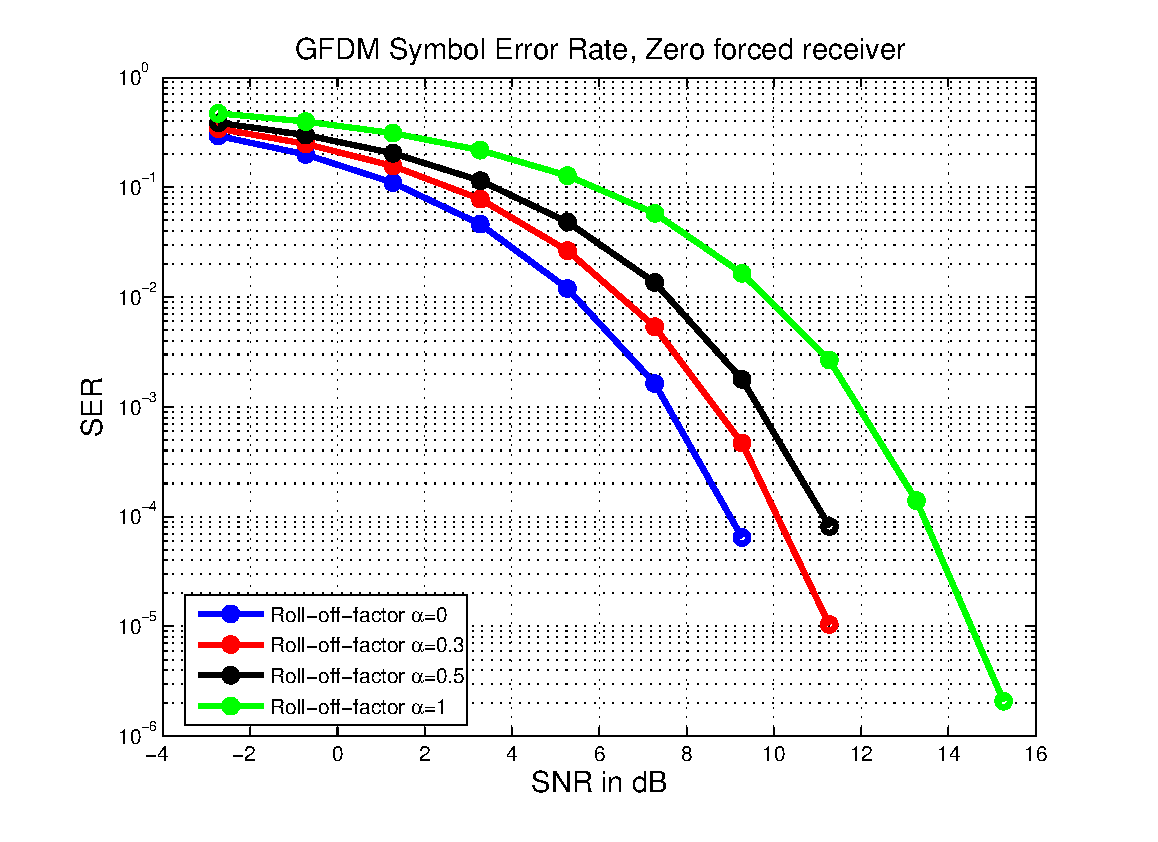
\includegraphics[width=0.9\columnwidth]{ZF_SER.eps}
\caption{\textit{SER dependency from $\alpha$ roll-off factor. Zero-forced receiver}}
\label{fs_1}
\end{figure}
\begin{figure}[H]
\centering
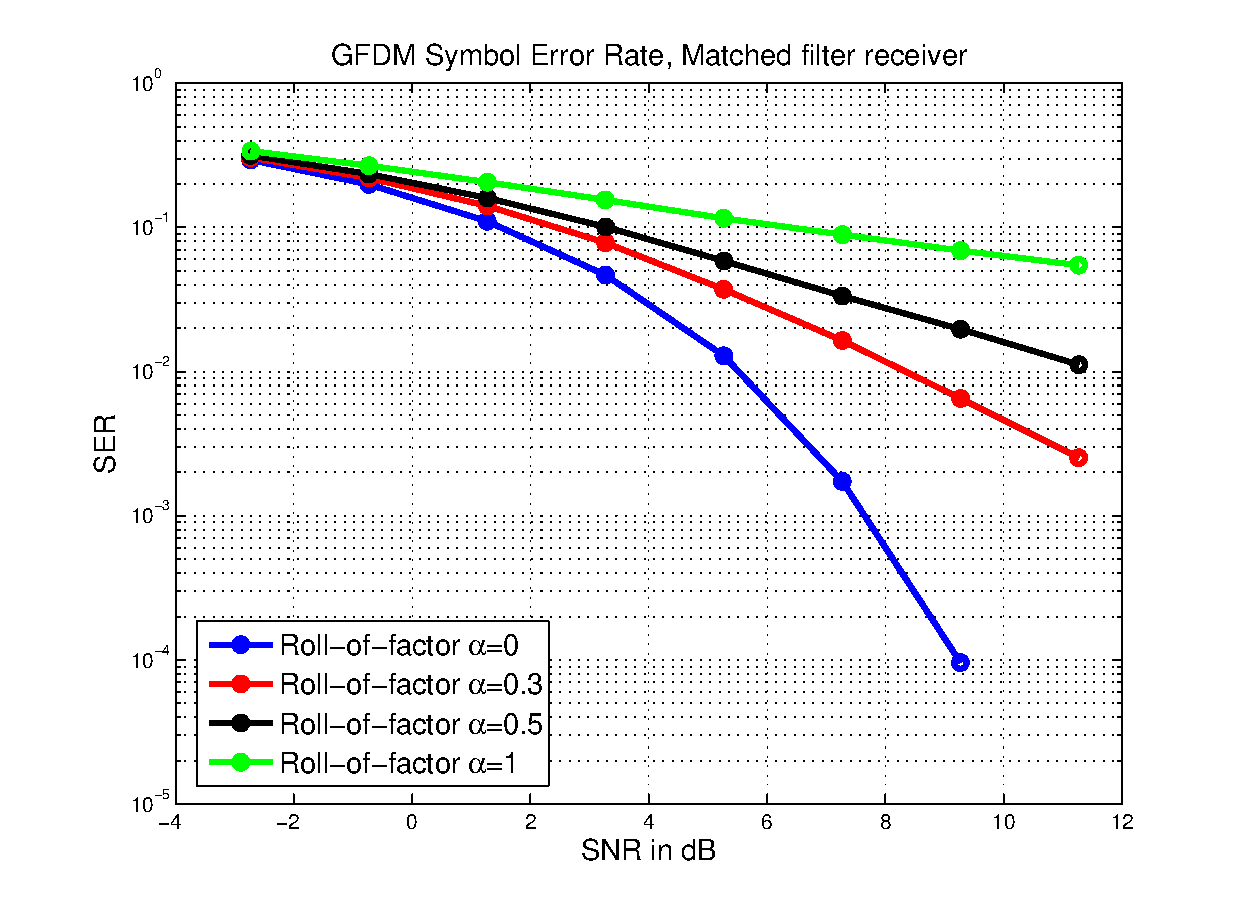
\includegraphics[width=0.9\columnwidth]{MF_SER.eps}
\caption{\textit{SER dependency from $\alpha$ roll-off factor. Matched filter receiver}}
\label{fs_2}
\end{figure}
\subsection{Scenario 1.2}
Performance results of the GFDM selection coefficient estimation and semi-blind receiver are obtained through simulation. The parameters of the system are tabulated in Table \ref{tab:table2}. 
\begin{table}[H]
\caption{\label{tab:table2}GFDM simulation parameters.Scenario 1.2}
\begin{center}
\begin{tabular}{|c|c|c|}
\hline
Parameter & Variable & GFDM \\
\hline
\hline
Modulation scheme & $\mu$ & QPSK \\
\hline
Samples per symbol & $T/T_s$ & 32 \\
\hline
Sub-carriers&$F$&32 \\
\hline
Block size& $T_s$  &15 \\
\hline
Filter type&  &RRC \\
\hline
Roll-off-factor&$\alpha$  &0.5 \\
\hline
Sub-carrier coefficients& $\mathbf{a}_i$ & $unif(0,1)$ \\
\hline
Channel& $h$ &AWGN \\
\hline
Cyclic Prefix&  & No \\
\hline
Transmission&  & Uncoded\\
\hline
\end{tabular}
\end{center}
\end{table}
The GFDM system is simulated with AWGN channel. QPSK modulation scheme is used. The number of sub-carriers was $F=32$, samples for each symbol was $T/T_s=F$ The block size was $T_s=15$. The root-raised cosine filter was used with roll-of-factor $\alpha=0.5$. The selection coefficients was chosen as the random integer values in range from $0$ to $1$.  The results of the GFDM performance is presented in the two plots, at first \eqref{fs_3} is shown the SER in comparison with the case  if receiver know the original $\mathbf{a}$ with the Zero-Forced receiver and with case if receiver doesn't know the $\mathbf{a}$ . At second figure \eqref{fs_4} is shown the reconstruction error for the $\mathbf{a}$ .
\begin{align}
r=\frac{\mid\mid\mathbf{\widehat{a}}-\mathbf{a}\mid\mid^2}{\mid\mid\mathbf{a}\mid\mid^2}
\end{align}
\begin{figure}[H]
\centering
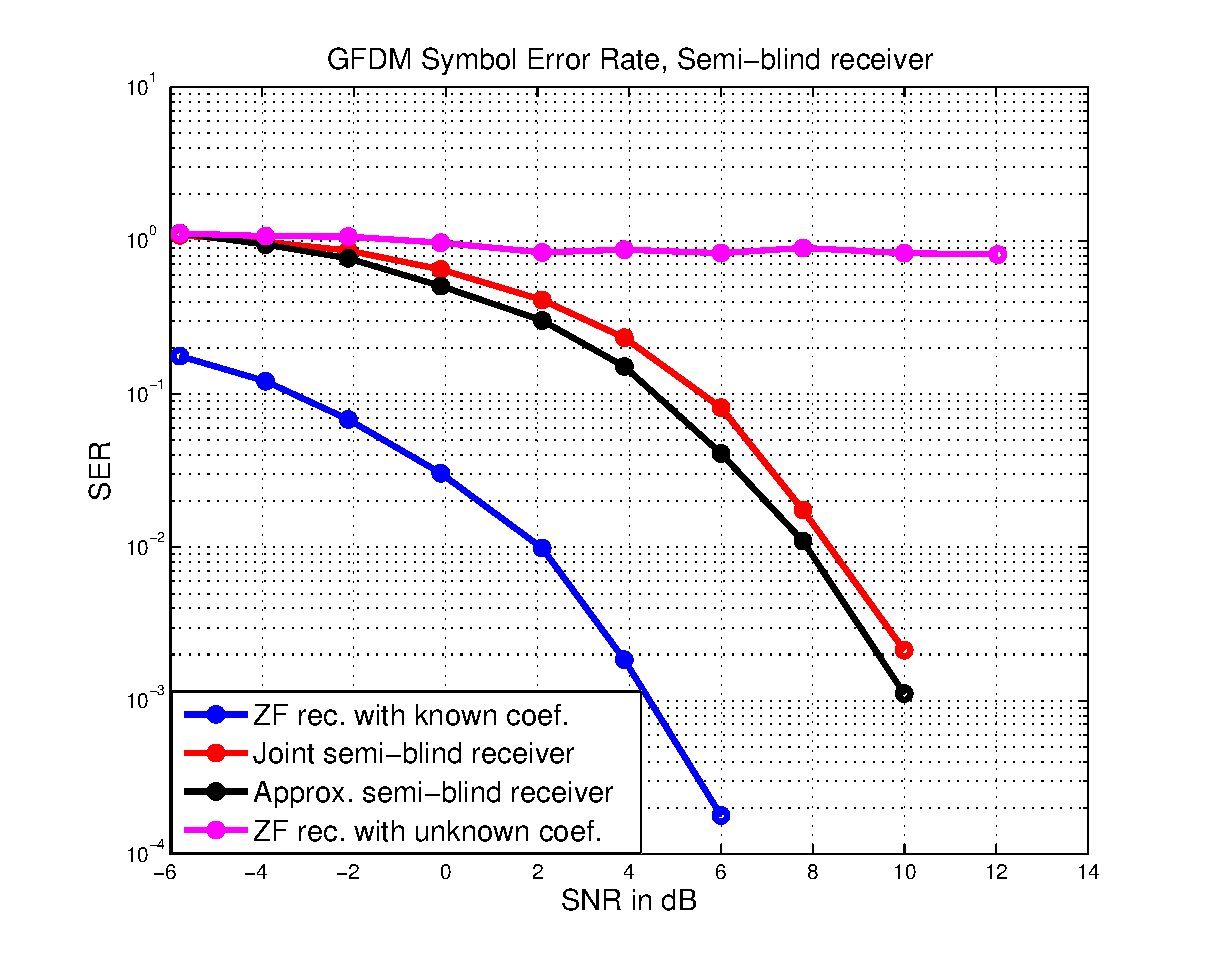
\includegraphics[width=0.9\columnwidth]{SM_SER.eps}
\caption{\textit{SER comparison for the semi-blind and zero-forced receiver}}
\label{fs_3}
\end{figure}
\begin{figure}[H]
\centering
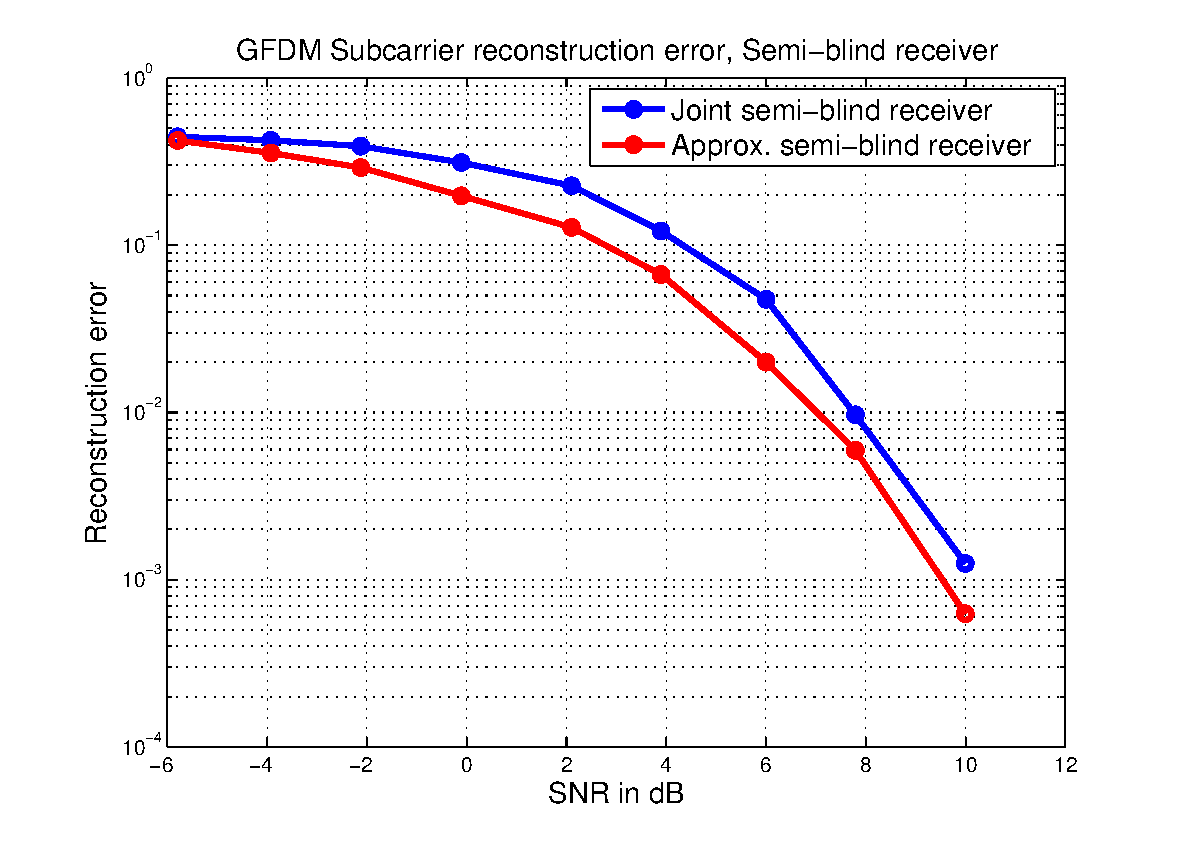
\includegraphics[width=0.9\columnwidth]{SM_RE.eps}
\caption{\textit{Reconstruction error for the semi-blind receiver}}
\label{fs_4}
\end{figure}
\subsection{Scenario 1.3}
There are additional plots for the joint and approximated algorithms comparison is shown at  fig.\eqref{fs_5} fig.\eqref{fs_6} fig.\eqref{fs_7}. The comparison results are obtained through simulation. The simulation set-up is shown in the Table \ref{tab:table3}.The GFDM system is simulated with AWGN channel. QPSK modulation scheme is used. The parameters of the setup is the same as in the previous experiment. In the fig.\eqref{fs_5} is shown the typical reconstruction error convergence of the both of the algorithms per iterations. As the real minimum point is shown values of the residual between generated matrices and received data. In the fig.\eqref{fs_6} shown the time of the convergence of the algorithm with dependence for the SNR. In the fig.\eqref{fs_7} shown the typical convergence of the residual \eqref{sim:eq_1} of the both of the algorithms per iterations.
\begin{align}
\mathbf{r}_1^H\mathbf{r}_1= (vec(\mathbf{y})-\mathbf{\Omega}_1 \cdot vec(\mathbf{\widehat{S}}) )^H(vec(\mathbf{y})-\mathbf{\Omega}_1 \cdot vec(\mathbf{\widehat{S}}) )
\label{sim:eq_1}
\end{align}
\begin{table}[H]
\caption{\label{tab:table3}GFDM simulation parameters.Scenario 1.3}
\begin{center}
\begin{tabular}{|c|c|c|}
\hline
Parameter & Variable & GFDM \\
\hline
\hline
SNR & $log(P_s/P_n)$ & 10 \\
\hline
Samples per symbol & $T/T_s$ & 32 \\
\hline
Sub-carriers&$F$&32 \\
\hline
Block size& $T_s$  &15 \\
\hline
Filter type&  &RRC \\
\hline
Roll-off-factor&$\alpha$  &0.5 \\
\hline
Sub-carrier coefficients&$a_i$& $unif{0,1}$ \\
\hline
\end{tabular}
\end{center}
\end{table}
\begin{figure}[H]
\centering
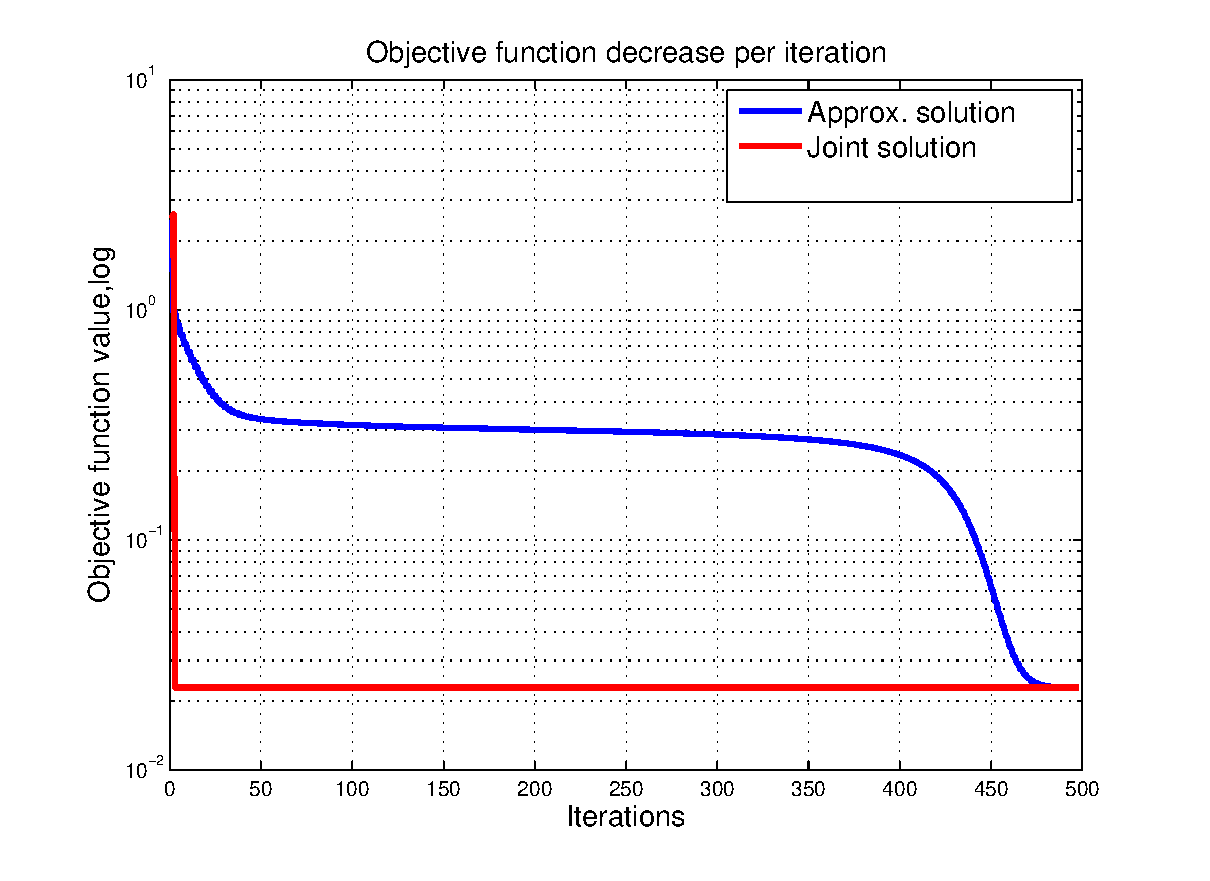
\includegraphics[width=0.9\columnwidth]{SM_conv.eps}
\caption{\textit{Convergence of the semi-blind receiver with respect to the iterations}}
\label{fs_5}
\end{figure}

\begin{figure}[H]
\centering
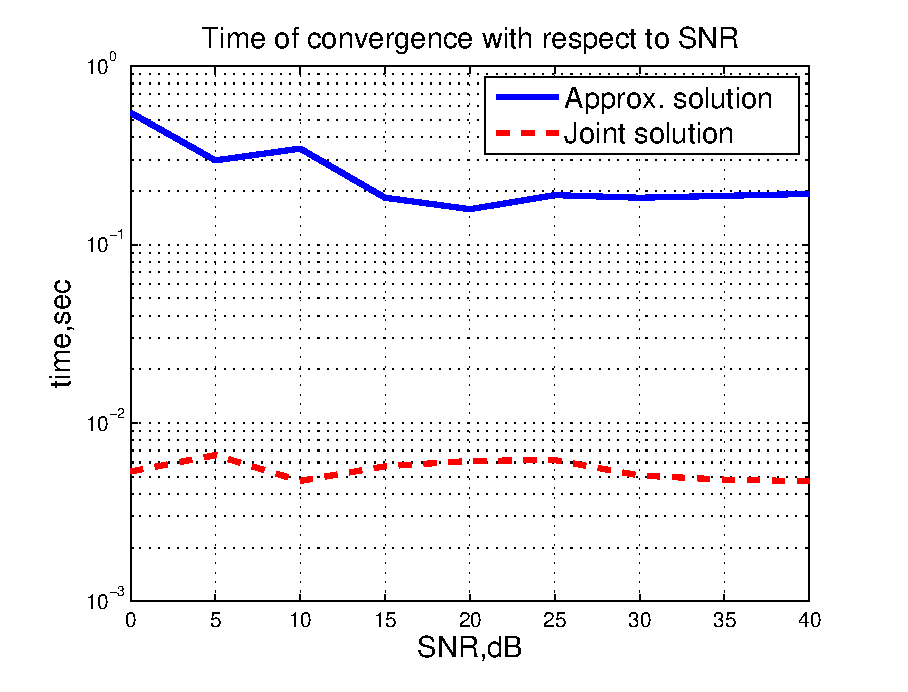
\includegraphics[width=0.9\columnwidth]{SM_TIME.eps}
\caption{\textit{Convergence time for the semi-blind receiver with respect to the SNR}}
\label{fs_6}
\end{figure}
\begin{figure}[H]
\centering
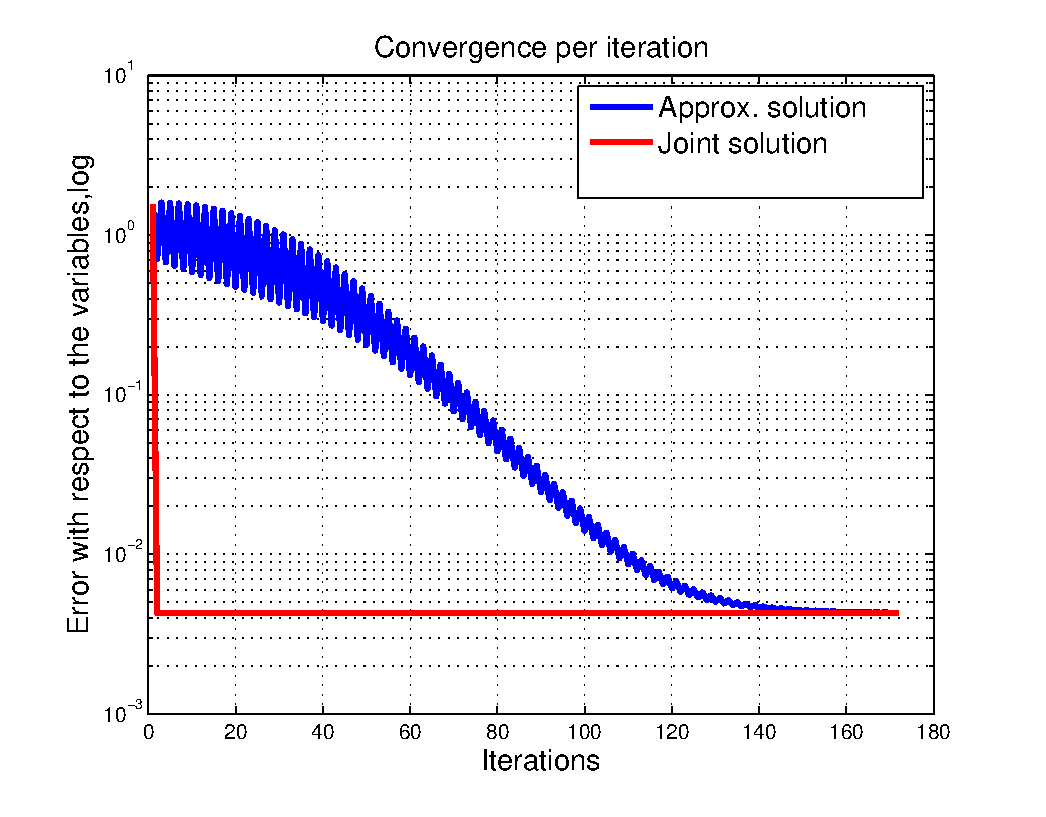
\includegraphics[width=0.9\columnwidth]{SM_RES.eps}
\caption{\textit{Residual decrease for the semi-bind receiver with respect to the iterations}}
\label{fs_7}
\end{figure}
\subsection{Scenario 1.4}
\begin{table}[H]
\caption{\label{tab:sisotable5}GFDM simulation parameters.Scenario 1.4}
\begin{center}
\begin{tabular}{|c|c|c|}
\hline
Parameter & Variable & GFDM \\
\hline
\hline
Modulation scheme & $\mu$ & QPSK \\
\hline
Samples per symbol & $T/T_s$ & 32 \\
\hline
Sub-carriers&$F$&32 \\
\hline
Block size& $T_s$  &15 \\
\hline
Filter type&  &RRC \\
\hline
Roll-off-factor&$\alpha$  &1 \\
\hline
Channel& $h$ & Ped-A \\
\hline
Length of the channel& $L+1$ & 12 \\
\hline
Cyclic Prefix&  & No \\
\hline
Transmission&  & Uncoded\\
\hline
\end{tabular}
\end{center}
\end{table}
The GFDM system semi-blind receiver is simulated in the frequency selective channel without coding. QPSK modulation scheme is used. The number of sub-carriers was $F=32$, samples for each symbol was $T/T_s=F$ The block size was $T_s=15$. The root-raised cosine filter was used with roll-of-factor $\alpha=1$. The length of the channel equal to $L+1=12$. The values of the channel is presented in the table \ref{tab:sisotable5}. The results of the GFDM performance are presented in the two plots, at first \eqref{fs_8} is shown the SER in comparison with the Zero-Forcing FFT receiver and with case for different number of unknown symbols in one transmission block. In the simulation we define as the unknown symbol number of the non-training symbols in the $vec(\mathbf{S})$ At second figure \eqref{fs_9} is shown the reconstruction error for the channel.
\begin{figure}[H]
\centering
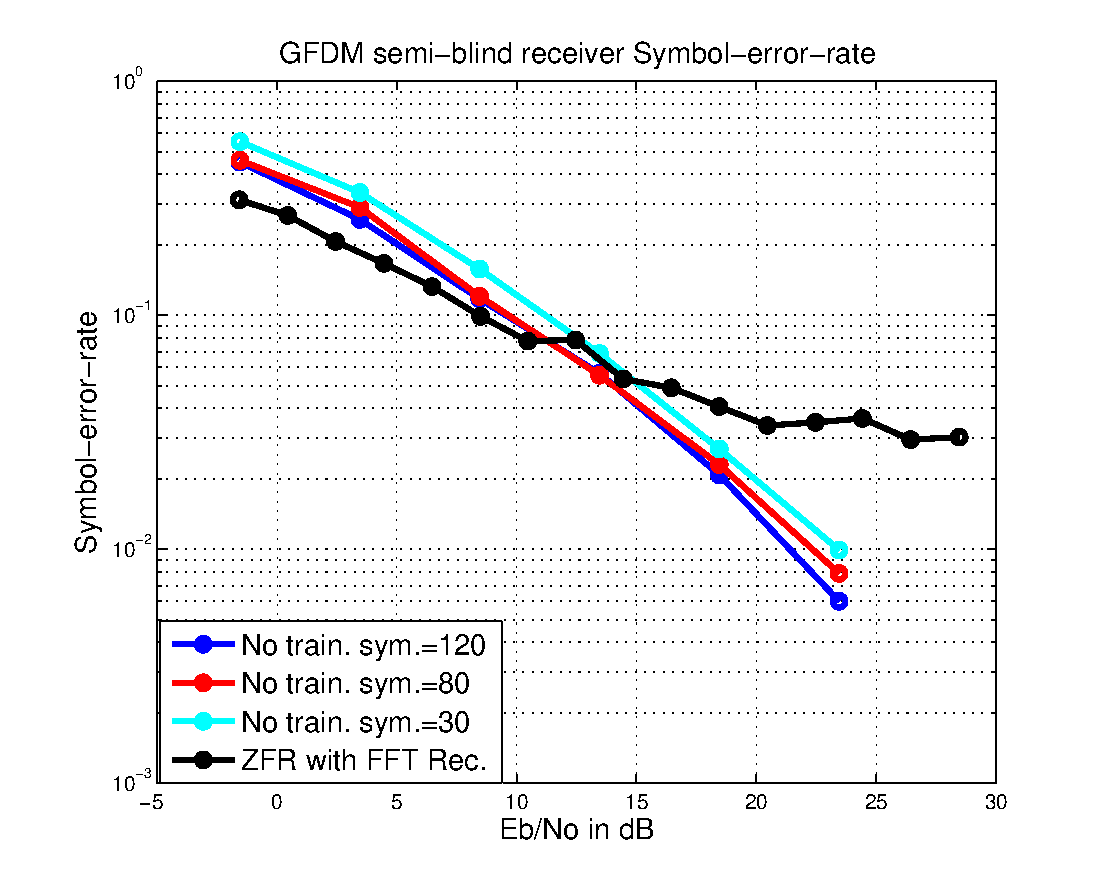
\includegraphics[width=0.9\columnwidth]{SM_SISO_FS_SER.eps}
\caption{\textit{SER for the semi-blind receiver with different number of known symbols}}
\label{fs_8}
\end{figure}
\begin{figure}[H]
\centering
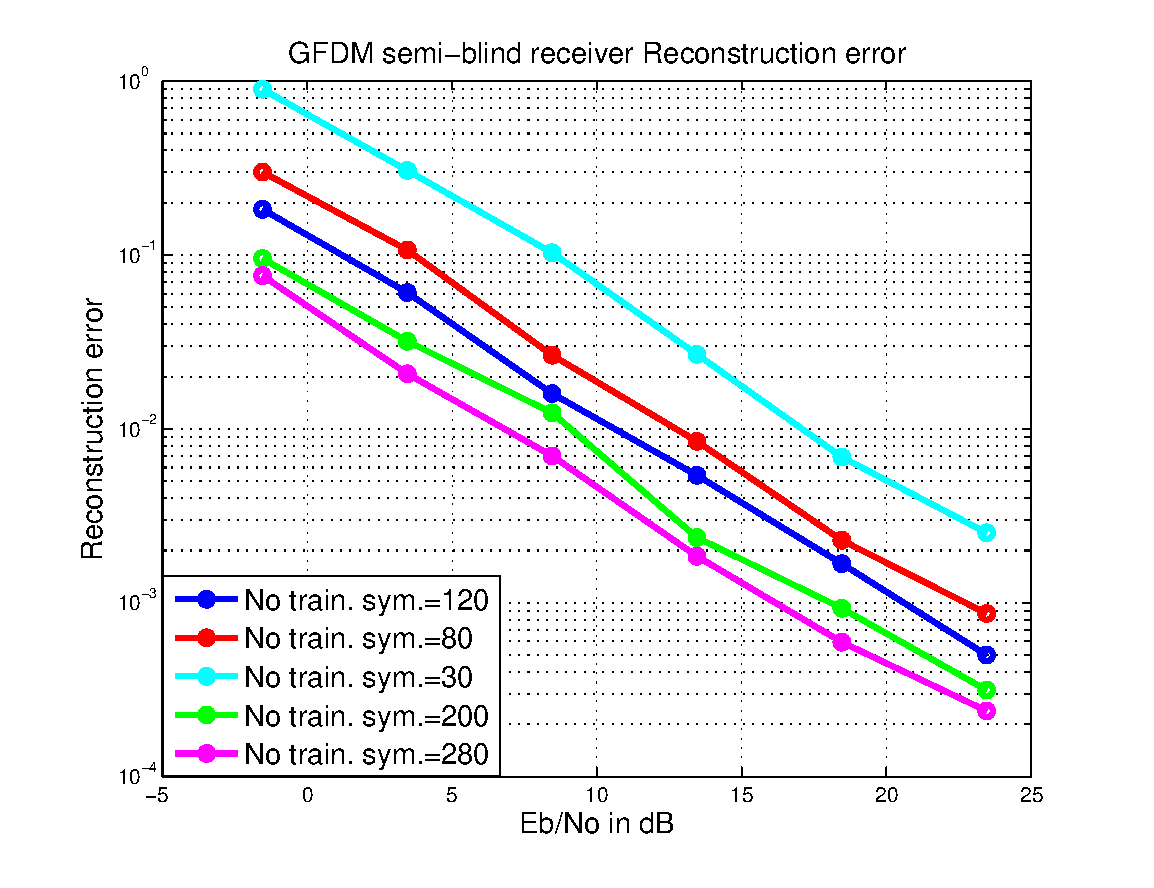
\includegraphics[width=0.9\columnwidth]{SM_SISO_FS_RE.eps}
\caption{\textit{Channel reconstruction error for the semi-blind receiver with different number of known symbols}}
\label{fs_9}
\end{figure}
\section{Conclusion}\label{part:CSISO}
As conclusion for the first experiment we  can say that zero forced receiver show much better results in the symbol detection in comparison with matched filter. The difference become significant when the $roll-off$ factor of the $RRC$ filter increase. The ZF receiver has increased the SER slightly with $\alpha$ increasing which is shown at the fig.\ref{fs_1}. The MF receiver increase SER significantly  with $\alpha$ increasing which is shown at fig.\ref{fs_2}. Explained results show, that ZF receiver should be preferred in the receiver. The ZF receiver achieve the better performance with the same self-interference ratio and allow decreasing the out-of-band radiation. In general, even if we consider the noise enhancement from the ZF receiver, the performance of the system is much better in case if we use the ZF receiver. The MF receiver is much more depend from the $roll-off$ factor and has performance reduction due to this. 

As conclusion for the experiment with frequency coefficient selection approach we can see that algorithm decrease performance in comparison with system where  the frequency coefficients is known fig.\ref{fs_3}. Huge performance decrease come from the non-convenient coefficient selection way.We chose coefficient as $1$ if the resulting $abs(a_1)$ value is higher than $0.5$. There are better solutions to increase performance of the algorithm. We can use predefined information at the receiver. We can see that joint algorithm has slightly worse performance in symbol and frequency coefficients detection fig.\ref{fs_3}fig.\ref{fs_4}in comparison with approximated algorithm. This behaviour is explained from the initial point setup in the approximated algorithm. We take as the initially transmission coefficients equal to the zero. The approximated algorithm turn on less sub-carriers and make false negative errors. The false negative error lead to the better SER performance due to less estimated number of the symbols. The possible performance increase for the joint solution algorithm is the different weights for the objective function parts. The part for frequency coefficients estimations should have higher weight.

The next figures show advantages of the joint algorithm. As we can see from the fig. \ref{fs_5},fig.\ref{fs_6},fig.\ref{fs_7}. The residual decrease show that joint algorithm converge much faster than approximated. The typical number of iteration of the joint algorithm equal to $2$ and for the joint algorithm equal to the $200$. So significant difference neglect the difference between the computationally expensive iterations in the joint algorithm. The fig. \ref{fs_6} confirm that fact. The joint algorithm converge independently from the SNR and take 100 times less time to converge. The approximated algorithm slightly depend from the SNR in the received data.
The fig. \ref{fs_7} show that estimated values in the approximated algorithm decrease non-linearly. The shown fact mean that algorithm decrease at each iteration only one set of the variables, symbols or frequency coefficients. The overall conclusion is that approach is effective enough for the data estimation and there are possibility to increase performance with weights addition. Algorithm will show slightly better results if additional pre-processing will be used. The overall conclusion over the frequency coefficient algorithms we can say that spectrum sensing approach is applicable in the automatic way without a-priori information at the receiver. The receiver can estimate used subcarriers and estimate transmitted symbols with decrease in the performance. In the paper is explained very simple approach to coefficients estimation. Performance of the algorithm can be implemented in more efficient way without huge performance loss.

The next experiment show results of the semi-blind receiver. We estimated the unknown channel and the unknown symbols in the same time. We used the pedestrian-A type of frequency selective channel.  The result for the SER if shown in the fig. \ref{fs_8}. We can see from the results, algorithm show better performance in comparison with FFT receiver in the high SNR and slightly worse performance in the low SNR. The worse performance in the low SNR leads from the significant channel error estimation. We can see that performance in the FFT receiver has upper bound and FFT receiver doesn't allow to decrease the SER lower. This behavior leads from the rank of the channel matrix, which is not full. With the semi-blind receiver we can put the symbols in more convenient way to increase the performance of the algorithm. We can see that performance of the algorithm slightly depends from the number of training symbols. The difference from the number of used training symbols is not significant and equal to 2-3 dB. The fig.\ref{fs_9} show the reconstruction error of the channel estimation. We can see that channel estimation error has significant dependence from the number of training symbols. There is trade-off between channel estimation and the number of received information. As conclusion, we can say that semi-blind receiver allow to estimate the channel and the symbols without channel prefix, only with the known symbols in data block. The semi-blind receiver outperforms the FFT receiver. The disadvantage of the semi-blind receiver is computational complexity.

% As we can see here, there is one minimum point in symbol estimation. The less unknown symbols in the block leads to the SNR increase, whether the higher number of unknown symbols leads to the SER increase. The point where number of unknown symbols equal to $8$ show the closest result to the original GFDM system with the same block size but known channel and ZF receiver. The channel estimation error has the same behaviour and show the minimum point in the same number of unknown symbols. Important fact is that reconstruction error for the maximal and minimal number of unknown symbols have the same behaviour and lay in the same line. Which mean that maximum knowledge and maximal uncertainty show the same results. This behaviour also show the convexity of the performance function for the number of unknown symbols as variable. In the difference block size should be different optimal value of the unknown symbols, but the average performance must be the worse in comparison with the original GFDM system due to the higher energy per bit with same performance. There is additional important performance gain in the explained algorithm, the algorithm decrease the self-interference in the system from known symbols. The algorithm also can be written for the overall interference decrease, but better to use this algorithm after the semi-blind receiver.
